%%%%%%%%%%%%%%%%%%%%%%%%%%%%%%%%%%%%%%%%%
% Developer CV
% LaTeX Template
% Version 1.0 (28/1/19)
%
% This template originates from:
% http://www.LaTeXTemplates.com
%
% Authors:
% Jan Vorisek (jan@vorisek.me)
% Based on a template by Jan Küster (info@jankuester.com)
% Modified for LaTeX Templates by Vel (vel@LaTeXTemplates.com)
%
% License:
% The MIT License (see included LICENSE file)
%
%%%%%%%%%%%%%%%%%%%%%%%%%%%%%%%%%%%%%%%%%

%----------------------------------------------------------------------------------------
%	PACKAGES AND OTHER DOCUMENT CONFIGURATIONS
%----------------------------------------------------------------------------------------

\documentclass[9pt]{developercv} % Default font size, values from 8-12pt are recommended

%\usepackage{pstricks}
%\usepackage{pst-grad}
%\usepackage{multido}
%\usepackage{calc}
%\usepackage{fp-snap}
%\usepackage{ifthen}
%\usepackage{bardiag}
\usepackage{hyperref}
\usepackage{graphicx}

% Defining color variables
\definecolor{ballblue}{rgb}{0.13, 0.67, 0.8}
\definecolor{bleudefrance}{rgb}{0.19, 0.55, 0.91}

%----------------------------------------------------------------------------------------

\begin{document}

%----------------------------------------------------------------------------------------
%	TITLE AND CONTACT INFORMATION
%----------------------------------------------------------------------------------------

\begin{minipage}[t]{0.45\textwidth} % 45% of the page width for name
	\vspace{-\baselineskip} % Required for vertically aligning minipages
	
	% If your name is very short, use just one of the lines below
	% If your name is very long, reduce the font size or make the minipage wider and reduce the others proportionately
	\colorbox{black}{{\HUGE\textcolor{white}{\textbf{\MakeUppercase{Ernesto}}}}} % First name
	
	\colorbox{black}{{\HUGE\textcolor{white}{\textbf{\MakeUppercase{González}}}}} % Last name
	
	\vspace{6pt}
	
\end{minipage}
\begin{minipage}[t]{0.250\textwidth} % 27.5% of the page width for the first row of icons
	\vspace{-\baselineskip} % Required for vertically aligning minipages
	
	% The first parameter is the FontAwesome icon name, the second is the box size and the third is the text
	% Other icons can be found by referring to fontawesome.pdf (supplied with the template) and using the word after \fa in the command for the icon you want
	\icon{MapMarker}{12}{Lisbon}\\
	\icon{Phone}{12}{+351 935 117 765}\\

\end{minipage}
\begin{minipage}[t]{0.300\textwidth} % 27.5% of the page width for the second row of icons
	\vspace{-\baselineskip} % Required for vertically aligning minipages
	
	% The first parameter is the FontAwesome icon name, the second is the box size and the third is the text
	% Other icons can be found by referring to fontawesome.pdf (supplied with the template) and using the word after \fa in the command for the icon you want

\icon{At}{12}{\href{mailto:ernestogonzalezz@yahoo.com}{ernestogonzalezz@yahoo.com}}\\	
	\icon{Instagram}{12}{\href{}{@ernestofergo}}\\
\end{minipage}

\vspace{0.5cm}

%----------------------------------------------------------------------------------------
%	INTRODUCTION, SKILLS AND TECHNOLOGIES
%----------------------------------------------------------------------------------------
\cvsect{Description}
\begin{description}
	\item[Nationality]: cuban
	\item[Height]: 1.84 m
	\item[Weight]: 80 kg
	\item[Position]: Right Wing
\end{description}

%----------------------------------------------------------------------------------------
%	EXPERIENCE
%----------------------------------------------------------------------------------------
%\cvsect{Experience}

%\begin{entrylist}
%	\entry
%		{2017 -- 3/2018}
%		{Front-end developer}
%		{Big Corporation Name Inc.}
%		{\lorem \lorem \lorem\\ \texttt{node.js}\slashsep\texttt{Vue.js}\slashsep\texttt{Electron}}
%\end{entrylist}

%----------------------------------------------------------------------------------------
%	EDUCATION
%----------------------------------------------------------------------------------------
\cvsect{Youth}

\begin{entrylist}
	\entry
			{2010 - 2012}
		{BM Torrevieja sub-12}
		{Torrevieja, Spain}
		{2nd place Province of Alicante}
	\entry
			{2014-2015}
		{Sporting de Luanda sub-17}
		{Luanda, Angola}
		{6th place Province of Luanda}
	\entry
			{2015-2016}
		{BM Torrevieja sub-16}
		{Torrevieja, Spain}
		{2nd place Province of Alicante, Top 8 Comunitat Valenciana}
	\entry
			{2016-2018}
		{Sporting of Lisbon sub-18 and sub-20}
		{Lisbon, Portugal}
		{\begin{itemize}
		\item 1st place Lisbon District 2nd Division,
		\item 2nd place South Zone Portugal 2nd Division,
		\item 1st place Portugal National Championship sub-18 2017-2018,
		\item 1st place 2017 Penedono Tournament,
		\item 1st place 2018 Sassoeiros Tournament,
		\item 5th place Portugal National Championship sub-20 2016-2017.
		\end{itemize}}
	\entry
				{2018-2019}
		{CF Belenenses sub-20 and senior}
		{Lisbon, Portugal}
		{Top 6 Portugal National Championship sub-20}
	
\end{entrylist}

\cvsect{History}
To check my game history in Portugal visit \quad \url{http://portal.fpa.pt/fap_portal/do?COM=DS;1;111;+PAGE(2000054)+COD_COR_CAIXA(3)+K-CATEGORIA()+K-ID(293928)+RCNT(10)}


\begin{figure} [h]
\center
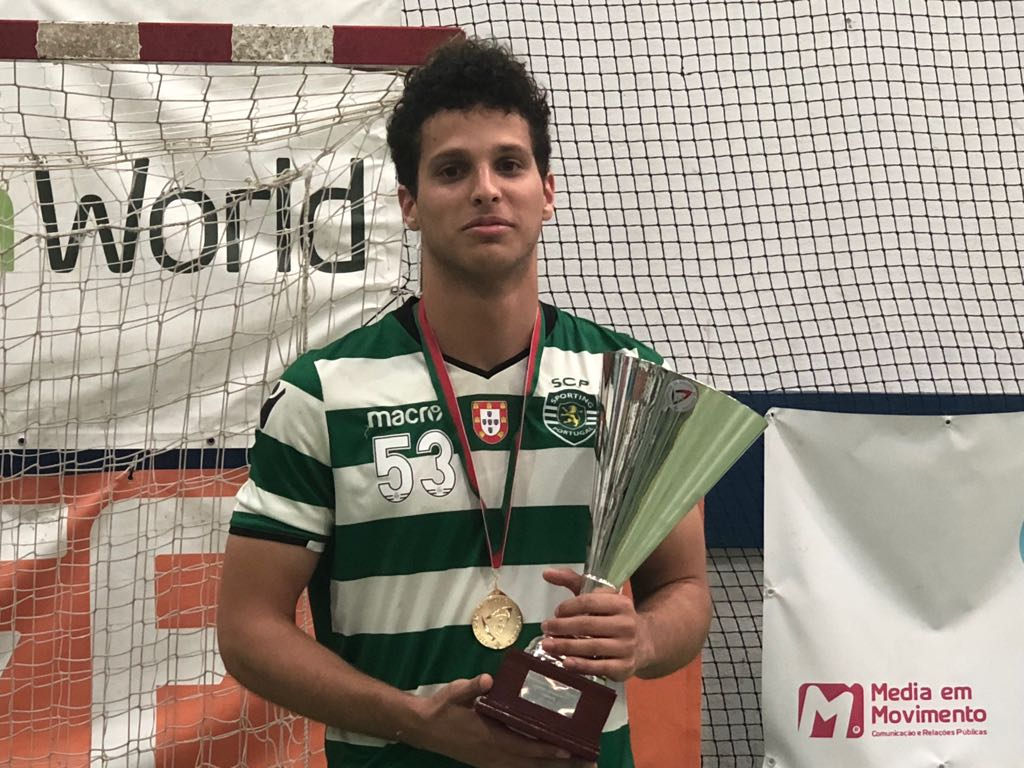
\includegraphics[scale=0.2]{eu}
\end{figure}

%----------------------------------------------------------------------------------------
%	ADDITIONAL INFORMATION
%----------------------------------------------------------------------------------------
%\begin{minipage}[t]{0.3\textwidth}
%	\vspace{-\baselineskip} % Required for vertically aligning minipages
%
%\cvsect{Projects}
%
%\begin{description}
%	\item \textbf{Meeting app website} full-stack
%	\item \textbf{Multiple Social Media Websites}: Twitter clone, blog, group chats...
%	\item \textbf{Trip Booking Website} front-end
%\end{description}
%\end{minipage}
%\hfill

%----------------------------------------------------------------------------------------

\end{document}
